\begin{frame}
  \frametitle{The full system}
  \begin{columns}
  \column{0.5\textwidth}
    \begin{itemize}
	\item Beagle Bone Black board (of course). The Wireless variant
	      should work fine too.
	\item Beagle Bone LCD cape\\
              \url{https://elinux.org/Beagleboard:BeagleBone_LCD4}\\
	      Unfortunately, no longer manufactured. You could adapt
	      the course to use an HDMI display instead.
        \item Standard USB webcam (supported through the \code{uvcvideo}
	      driver.
    \end{itemize}
  \column{0.5\textwidth}
     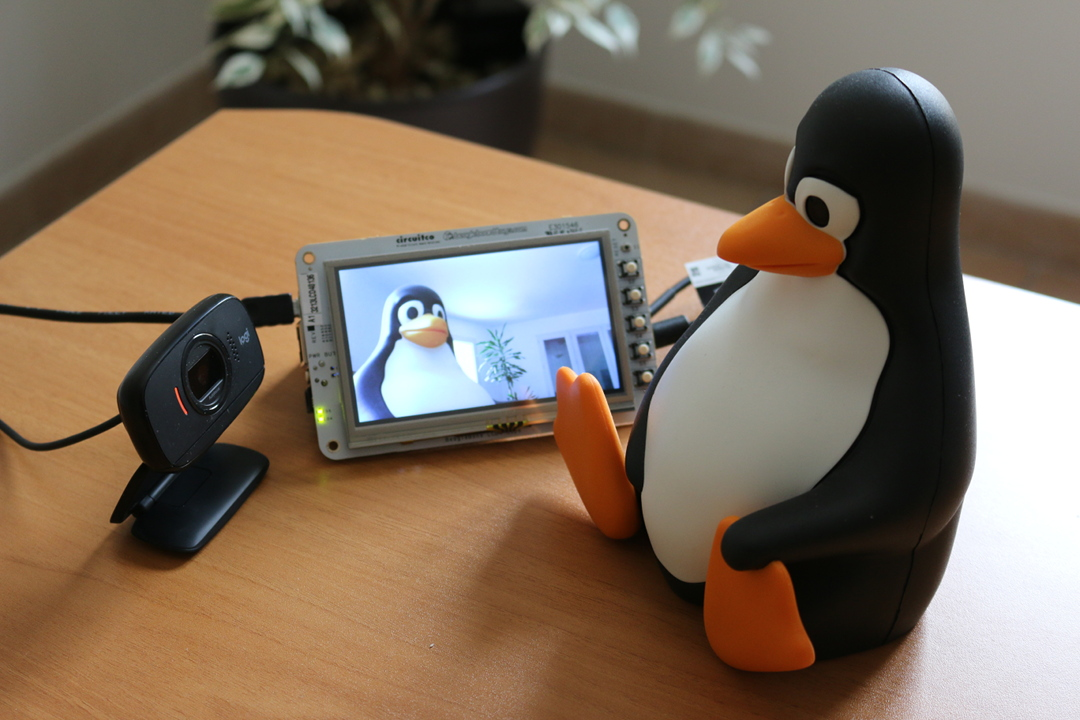
\includegraphics[width=\textwidth]{common/beaglecam.jpg}
  \end{columns}
\end{frame}



